\documentclass[12pt,a4paper]{article}
\usepackage[UTF8]{ctex}
\usepackage[backend=bibtex]{biblatex}
\usepackage{amsmath,amsthm,amssymb,graphicx,multirow,float,caption}
\usepackage{geometry}
\geometry{left=2.54cm, right=2.54cm, top=3.18cm, bottom=3.18cm}
\usepackage{enumitem}
\usepackage{subcaption,booktabs,diagbox}
\setenumerate[1]{itemsep=0pt,partopsep=0pt,parsep=\parskip,topsep=5pt}
\setitemize[1]{itemsep=0pt,partopsep=0pt,parsep=\parskip,topsep=5pt}
\setdescription{itemsep=0pt,partopsep=0pt,parsep=\parskip,topsep=5pt}
\usepackage{adjustbox}
\usepackage[graphicx]{realboxes}
\usepackage{rotating}
\usepackage{threeparttable}
\usepackage{titlesec}

\titleformat{\section}%设置section的样式
{\raggedright\large\bfseries}%右对齐,4号字,加粗
{\thesection .\quad}%标号后面有个点
{0pt}%sep label和title之间的水平距离
{}%标题前没有内容

\title{\vspace{-4cm}\Large 光纤的物理性质与应用}  %文章标题
\author{\kaishu 学号:202111999064 \hspace{2cm} 姓名:郑力恒}   %作者的名称
\date{}

\begin{document}
\maketitle

\begin{abstract}
    本实验关注光纤本身的性质. 这些性质既包括光纤材料固有的性质, 如折射率, 也包括光纤进行光学接触时表现出来的实验性质, 如
    光源与光纤的耦合效率, 光纤的数值孔径, 光纤的损耗等. 在本实验中, 我们测量了塑料光纤的耦合效率与损耗系数, 石英光纤的数值孔径. 基于双光源干涉, 观察并测量了
    石英光纤折射率随温度的变化. 

    \bf{关键词}: 光纤\quad 损耗系数\quad 温度系数
\end{abstract}

\section{引言}


光纤的起源追溯到贝尔光电话, 但其真正开始发展, 是由于激光的出现, 以及华人物理学家高锟指出的, 通过降低玻璃纤维中的杂质以获得可使用的光导纤维的制备方法. 因此, 降低杂质, 与减小
损耗系数, 是光纤工业持续的主题. 由于出色的低损耗性能, 光纤传输距离远, 信号稳定性好. 由于材料特性, 光纤成本
低, 寿命长, 耐腐蚀. 由于以光波作为信息载体, 光线的通信容量大. 因而在通信传输领域, 光纤是最佳的信息通道之一. 作为光纤发展的主题之一, 本实验
尝试对塑料光纤的损耗系数进行测量, 一并测量的还有光纤的耦合效率. 

光纤的另一个用途是传感器技术. 使用待测物理量对光纤中的光波进行调制, 在光学探测器中进行解调, 可以获得待测物理量变化的信息. 光纤作为传输介质时, 则具有
损耗低, 信息量大等优点. 本实验将使用石英光纤测量石英折射率随温度的变化. 折射率通过调制相位, 来改变光学探测器中的输出.


\section{原理}

\subsection{光源与光纤的耦合效率}
激光器输出的高斯光束, 经过透镜耦合之后, 与纤芯接触. 这里存在一个最佳的接触方式, 在理论上是
高斯光束的束腰与纤芯相匹配, 在实验上表现为光纤另一端出现最大的输出光强. 在此基础上, 在光纤端面入射的激光与透射进入光纤介质的激光仍有功率
上的不同. 因而, 可以定义耦合效率$\gamma$: 
\begin{equation}
    \gamma=\frac{P}{P_0}
\end{equation}

其中, $P_0$是入射到光纤端面的光功率, $P$是经耦合后输入光纤中的光功率. 
\subsection{光纤的数值孔径}
光纤的基础原理是全反射, 这就要求一个临界的入射角度. 事实上, 要实现全反射, 对入射角的最大值$\theta_{max}$有一个限制. 
这个角度值表征了光纤会聚光的能力. 在光纤的另一端, 由于光路的可逆性, 同样存在一个出射角的最大值, 大致上呈现圆锥的形式, 可以在远处测量光斑. 
通过在观察屏上测量光斑的半径$r$和光纤出射端面与观察屏的距离$h$, 可以求出这个最大值的正弦值, 并将其命名为光纤的数值孔径:
\begin{equation}
    NA=\sin{\theta_{max}}=\frac{r}{\sqrt{r^2+h^2}}
\end{equation}

\subsection{光纤的损耗系数}
虽然光波在光纤中是全反射, 但并不是完全没有损耗. 光纤材料本身会带来两种固有损耗: 散射和吸收. 散射主要来自杂质微粒, 吸收则是光纤材料和杂质共有的. 
光纤的损耗在宏观上表现为, 随着传播距离的增加, 光功率的指数衰减, 即存在
\begin{equation}
    P(L)=P(0)\exp{(-\alpha(\lambda)L)}
\end{equation}

通过测量一段光纤中的$P(L)$和$P(0)$, 我们类比声学中的分贝, 类似的定义如下的损耗系数: 
\begin{equation}
    \alpha(\lambda)=\frac{10}{L}\lg{\frac{P(0)}{P(L)}}
\end{equation}

\subsection{光纤温度传感器}
光纤的折射率会对光波的相位进行调制. 而对相位信息进行测量, 最直接的方法就是使用双光束干涉. 为此, 准备两条材质相同的光纤, 其中一条作为参考臂, 不作任何变动, 
另一条作为探测臂, 通过改变其温度, 来影响最终的干涉条纹. 相位与材料的折射率与光纤的长度有简单的关系: 
\begin{equation}
    \phi(T)=\frac{2\pi}{\lambda}n(T)L(T)-\phi_0
\end{equation}
在温度变化时, 总是有下式:
\begin{equation}
\Delta \phi=\frac{2\pi}{\lambda}(L\Delta n + n \Delta L)
\end{equation}

\section{实验}
本节介绍实验的仪器、实验方法和主要实验过程.
\subsection{光源与塑料光纤的耦合效率以及塑料光纤的损耗系数}
在进行这一步实验之前, 需要先确认激光器是否水平, 激光束是否与光轴共轴, 激光束是否与通光孔共轴. 
通过移动光阑, 观察目镜处的反射, 调节五维调节架等可以进行大致上的调整. 精细的调整需要安装了光纤之后才能进行.

本实验中测量塑料光纤的耦合效率. 
1. 在测量之前, 需要先保证塑料光纤的切面是光滑且平整的. 

2. 使用铜管固定光纤的一端, 露出铜管大概2mm左右. 这个露出长度不能太长; 如果太长了会导致光纤明显下垂, 偏离激光器的光轴, 导致无法进行耦合.
光纤的另一端与光功率计相接触.

3. 通过微调五维调节架的上下与左右位置, 目镜与激光器的距离等, 使得光纤另一端的功率达到最大, 这个时候可以认为是最佳耦合.

4. 这时可以进行损耗系数的测量了. 损耗系数要求测量一段长度为L的光纤中入射处的光功率与出射的光功率. 这里的光功率不能是未经耦合的激光器的功率. 
为此我们选取一段长度合适的光纤, 其长度为L, 测量其末端出射的光功率. 这就是公式(4)中的$P(L)$. 测量完毕后将其剪下, 剩下一小段长度为l的光纤仍连接着铜管. 此时再次测量其末端出射的光功率. 由于l很小, 这一光功率可以认为是
经过耦合, 但没有损耗的光功率, 即为公式(4)中的$P(0)$.

5. P(0)作为经过耦合, 但没有损耗的光功率, 可以用于计算耦合系数, 即公式(1)中的$P$. 因而, 只需测量$P_{0}$
即可. 由于不便拆卸五维调节架进行直接测量, 这里将铜管取下, 使用光功率计测量经过通光孔出射的光强, 近似代替无耦合的激光器功率, 即$P_{0}$.

至此, 就完成了所有需要的物理量的测量. 

\subsection{石英光纤的数值孔径}
测量数值孔径时采用的方法, 是远场光斑法. 我们需要在距离光纤出射端面一定距离以外的观察屏上观察到比较清晰的光斑. 这就要求石英光纤与光源的耦合得比较好. 
为此, 需要更加精细地调节五维调节架和保证光纤端面的平整性. 

1. 取用较长的石英光纤, 使用剥线钳剥除其外表的黄色套塑, 白色涂敷层, 以及包层, 露出一段2cm左右的裸光纤. 

2. 在显微镜下观察裸光纤的端面是否平整; 如果不平整, 需要使用光纤切割器进行切割, 直到端面平整. 如果裸光纤的长度不足, 需要返回第一步, 重新进行剥除. 

3. 使用铜管, 在白色涂敷层处固定这一端光纤. 调整五维调节架的上下与左右. 在入射端面, 应能明显观察到激光集中在纤芯上, 出射的一端光强达到较大值, 即能在白纸上看到比较明显的光斑后, 
通过光功率计进行进一步的微调, 达到最佳的耦合. 

4. 达到最佳的耦合以后, 就能进行数值孔径的测量了. 将光纤的出射端水平固定. 调节观察屏与其等高. 测量出射端面到观察屏的距离h. 对于光斑的半径r, 由于
光斑并不是非常规整的圆形, 测量水平方向的直径和数值方向的直径, 并取平均来获得这一半径大小r, 带入公式(2)即可获得数值孔径. 

\subsection{光纤温度传感器}
基于双光束干涉的两束光纤, 要达到一个相对良好的衬比度, 最基本的要求是两束光尽可能的同向, 光强相近. 此外, 光强的绝对大小也很重要. 
1. 因此, 在最佳耦合的状态下, 将石英光纤的输出端输入分束-干涉系统. 
2. 在分束系统后面的4条光纤中选取光强相近的两条, 在保证端面平整的情况下, 其中一条作为参考臂, 其中一条作为探测臂. 探测臂需要穿过放入桌面上的加热器狭缝中并固定好. 
3. 参考臂和探测臂需要在CCD前端调整方向并固定. 调整CCD和光纤端面的相对位置使得显示屏幕上出现明显的干涉条纹. 
4. 开启加热器. 同时记录下温度与显示器上的干涉条纹变动. 在30°C-40°C的范围内, 升温与降温各测一次. 
5. 计算条纹变动数N随温度的变化率, 即温度系数: $\frac{\Delta n}{\Delta T}$. 并与公式(6)相比较.

\section{结果分析与讨论}
\subsection{塑料光纤的损耗系数和耦合系数}
本实验中待测的核心物理量有待测光纤的长度L, 入射端耦合后的光功率P(0), 出射端的光功率P(L), 通过通光孔后的光功率P.
使用的公式主要是
\begin{equation}
    \begin{aligned}
    \alpha(\lambda,L,P(0),P(L))&=\frac{A(\lambda)}{L}=\frac{10}{L}\lg{\frac{P(0)}{P(L)}}
    \\
    \gamma(P(0),P)&=\frac{P(0)}{P}
    \end{aligned}
\end{equation}
本实验中进行了3次测量, 实验数据与读数记录如下: 
\begin{table}[H]
    \centering
    \begin{tabular}{|c|c|c|c|c|c|c|} 
    \hline
      & L/cm  & P(0)/mW & P(L)/mW & P/mW & $\alpha$/(dB/km) & $\gamma$/\%  \\ 
    \hline
    1 & 186.7 & 0.683   & 0.564   & 1.71 & $445 \pm 534$                    & $40\pm 6  $                 \\ 
    \hline
    2 & 180.8 & 0.888   & 0.501   & 1.61 & $1374 \pm 550$                   & $55\pm 7 $                   \\ 
    \hline
    3 & 175.4 & 0.861   & 0.710    & 1.33 & $477 \pm 452 $                   & $65 \pm 9 $                  \\
    \hline
    \end{tabular}
    \caption{塑料光纤的损耗系数$\alpha$和耦合系数$\gamma$}
\end{table}


在上表中, 使用了如下公式进行不确定度的计算: 
\begin{equation}
    u(W)=\sqrt{\sum_{i=1}^N (u(x_{i})\frac{\partial W}{\partial x_{i}})^2}
\end{equation}
其中, 由于测量光纤长度L时不一定完全拉直, 取u(L)=0.5cm. 测量光功率(P(0),P(L),P)时, 不一定达到最佳耦合, 故取u(P)=0.1mW, 
而这只需要轻微扰动调节架就会达到. 

注意到$u(\alpha)$达到了500dB/km, 这几乎是$\alpha$本身的量级. 这一点其实并不意外. u($\alpha$)主要取决于u(P)的大小. 事实上, 如果取u(P)为0.01mW, $u(\alpha)$会来到相对理想的50dB/km, 但实际中
这么小的u(P)是很难达到的. 而即使取u(P)为0.05, u($\alpha$)也有250左右的大小.

于是, 综合三次实验数据, 我们得到$\alpha$的值在1000dB/km左右. $\gamma$的值在50\%左右.

\subsection{石英光纤的数值孔径}
本实验中待测的核心物理量有远场光斑的半径大小$r$, 光纤出射端面到观察屏的距离$h$. 
使用的公式主要是:
\begin{equation}
    NA(r,h)=\frac{r}{\sqrt{r^2+h^2}}
\end{equation}
在石英光纤调整至最佳耦合以后, 改变了h三次, 采集了半径r三次, 记录如下:
\begin{table}[H]
    \centering
    \begin{tabular}{|c|c|c|c|} 
    \hline
      & r/cm & h/cm & NA           \\ 
    \hline
    1 & 0.70  & 8.1  & $0.086\pm 0.012$  \\ 
    \hline
    2 & 0.57 & 5.5  & $0.103\pm 0.018$  \\ 
    \hline
    3 & 1.00   & 10.1 & $0.099\pm 0.010$  \\
    \hline
    \end{tabular}
    \caption{石英光纤的数值孔径NA}
    \end{table}
不确定度的计算公式仍然是公式(8). 其中, u(r)因为间接测量和除以2的缘故, 取为0.1cm, u(h)因为没用尺子精确地对齐, 取为0.2cm. 

综合三次测量, 得到石英光纤的数值孔径在0.1左右.

\subsection{光纤温度传感器的温度系数}
本实验中待测的物理量有$\Delta N$和$\Delta T$. 

在实验中, 测量了升温区间和降温区间各一段. 从直观性上看, 采用N-T的图表会好一些, 但由于一些原因, 这里不这么呈现: (1)
手机相机成像并不稳定, 选择的定标点有时候会突然模糊, 不便于持续定标; (2)在降温阶段, 可能是由于空调的工作, 实验室中说话, 在工作台上的其他操作等扰动, 导致出现了条纹的反复吞吐现象, 不便于
持续定标. 

所以报告中采用了区间定标, 即选取一段合适的区间, 定标点稳定的情况下, 条纹的吞吐现象不严重时进行测量. 测量数据如下表所示: 
\begin{table}[H]
    \centering
    \begin{tabular}{|c|c|c|c|c|} 
    \hline
    温度区间/(°C)                 & 30-31.3 & 33-36     & 37-40   & 40-37  \\ 
    \hline
    $\Delta N$ & 5.5     & 12        & 16.5    & 10     \\ 
    \hline
    温度区间/(°C)                 & 36-35.2 & 33.5-32.2 & 32-31.1 & 31-30  \\ 
    \hline
    $\Delta N$ & 3.5     & 11.5      & 4       & 2.5    \\
    \hline
    \end{tabular}
    \caption{选取合适的温度区间测量条纹变化数. 在区间的表示上, 如果左边的数小于右边, 则为升温区, 反之则为降温区}
    \end{table}
升温和降温情况下, 各区间的平均值与总体的比较, 可以在下图中看出来:

    \begin{figure}[H]
        \centering
        
        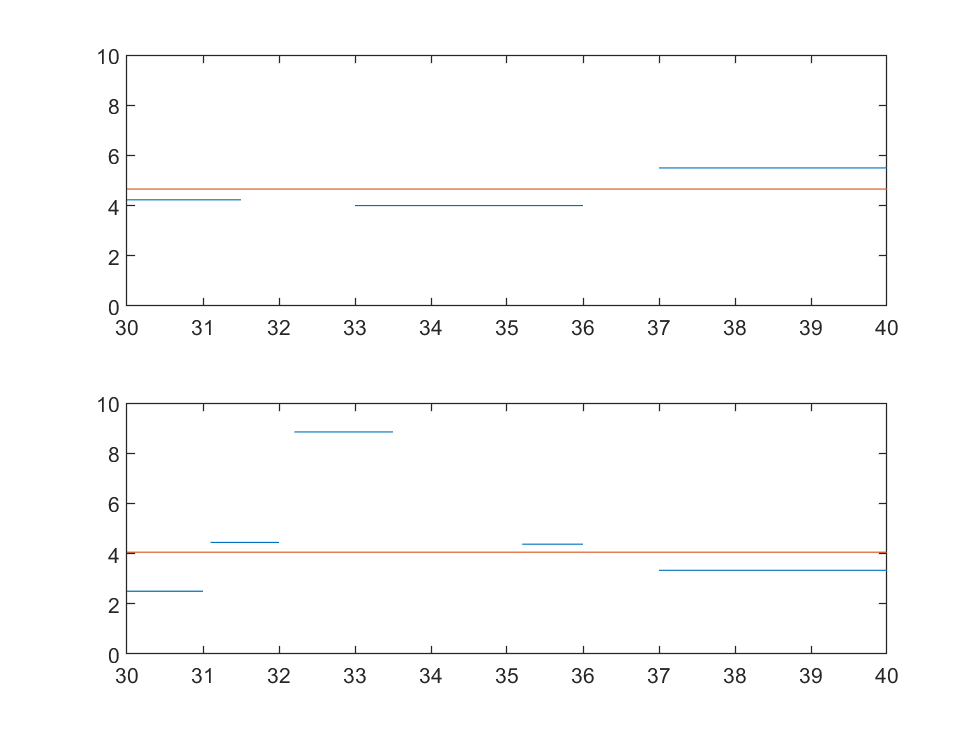
\includegraphics[width=0.6\textwidth]{fig1.png}
        \caption{升温和降温情况下, 各区间的平均值与总体的比较. 其中, 横坐标是温度, 纵坐标是计算出来的平均值. 
        上方的图是升温情况, 下方的图是降温情况. 蓝色的线是区间平均, 橙色的线则是总平均}
    \end{figure} 

可以看出, 由于降温区反复吞吐的现象存在, 降温情况下的温度系数方差极大. 例如降温情况中33.5°C-31.1°一段, 出现了条纹的快速移动. 因此在这一段便停止了定标. 之后的32°C-31.1°C和31°C-30°C
则呈现停滞或反复吞吐, 以致于正向的条纹移动数很少, 对前面一个区间进行了补偿. 


由于数据方差很大, 不确定度的计算没有太大意义. 升降温区各自测得的平均值为
\begin{equation}
    \begin{aligned}
        \frac{\Delta N}{\Delta T}_{\text{升}}&=4.66\text{条}/°C
        \\
        \frac{\Delta N}{\Delta T}_{\text{降}}&=4.06\text{条}/°C
    \end{aligned}
\end{equation}

此处可以和理论值相比较: 取石英的折射率为1.46, 探测臂被加热部分长度取为0.3m, 由于外层套塑的存在, 忽略石英的热膨胀, 
折射率温度系数取为$6.8 \times 10^{-6} /{ }^{\circ} \mathrm{C}$, 则可以计算出
\begin{equation}
    \frac{\Delta N}{\Delta T} = \frac{\Delta \varphi}{2 \pi \Delta T} = \frac{1}{\lambda}\left(L \frac{\Delta n}{\Delta T}\right) =4.7\text{条}/(°C)
 \end{equation}

但这个计算结果是在纯石英的情况, 仅忽略热膨胀系数时进行的. 实际情况中, 由于外层套塑导热性能差, 光纤与加热板固定的也不是很好, 最终实验值方差大, 同时理论值不完备, 数值相近只是巧合. 
但温度系数在$5\text{条}/(°C)$的量级应是没问题的. 
\section{总结和建议}
本实验中, 使用了截断法测量了塑料光纤的耦合系数(50\%), 塑料光纤的损耗系数(1000dB/km). 使用远场光斑法测量了石英光纤的数值孔径(0.1). 
最后, 通过双光束干涉法测量了光纤温度传感器的温度系数(5条/°C), 并和理论计算结果做了比较. 
\end{document}